% Generated by my modifications to the default Pandoc beamer template.
% Karl Browman has a tutorial about how to make Beamer sane:
% http://kbroman.wordpress.com/2013/10/07/better-looking-latexbeamer-slides/

% 12pt by default; handout if the handout template variable is defined
%\documentclass[12pt,ignorenonframetext,handout,12pt]{beamer}
\documentclass[12pt,handout]{beamer}
\usetheme{metropolis}

\providecommand{\tightlist}{%
  \setlength{\itemsep}{0pt}\setlength{\parskip}{0pt}}


% theme, colortheme, and fonttheme with sensible defaults
%%\usetheme{metropolis}
%%%\usecolortheme{dove}
%%
% if it is a handout show the notes text; otherwise don't
\setbeameroption{hide notes}
\setbeamertemplate{note page}[plain]

% Don't show things we don't want to see
\beamertemplatenavigationsymbolsempty
\hypersetup{pdfpagemode=UseNone} % don't show bookmarks on initial view

% Slide number in lower right
\definecolor{gray}{RGB}{155,155,155}
\setbeamertemplate{footline}{%
    \raisebox{5pt}{\makebox[\paperwidth]{\hfill\makebox[20pt]{\color{gray}
          \scriptsize\insertframenumber}}}\hspace*{5pt}}

% Space between paragraphs on notes page
\addtobeamertemplate{note page}{\setlength{\parskip}{12pt}}

% Color and shape of bullets
% \setbeamercolor{item}{fg=gray} 
% \setbeamercolor{subitem}{fg=gray}
% \setbeamercolor{itemize/enumerate subbody}{fg=gray}
\setbeamertemplate{itemize item}{{\textendash}}
\setbeamertemplate{itemize subitem}{{\textendash}}
\setbeamerfont{itemize/enumerate subbody}{size=\footnotesize}
\setbeamerfont{itemize/enumerate subitem}{size=\footnotesize}

\usepackage{amssymb,amsmath}
\usepackage{ifxetex,ifluatex}
\usepackage{fixltx2e} % provides \textsubscript
\ifxetex
  \usepackage{fontspec,xltxtra,xunicode}
  \defaultfontfeatures{Mapping=tex-text,Scale=MatchLowercase}
\else
  \ifluatex
    \usepackage{fontspec}
    \defaultfontfeatures{Mapping=tex-text,Scale=MatchLowercase}
  \else
    \usepackage[utf8]{inputenc}
  \fi
\fi
\usepackage{graphicx}
% Redefine \includegraphics so that, unless explicit options are
% given, the image width will not exceed the width of the page.
% Images get their normal width if they fit onto the page, but
% are scaled down if they would overflow the margins.
\makeatletter
\makeatother
\let\Oldincludegraphics\includegraphics
\renewcommand{\includegraphics}[2][]{\Oldincludegraphics[width=\textwidth,height=0.7\textheight,keepaspectratio]{#2}}

% Comment these out if you don't want a slide with just the
% part/section/subsection/subsubsection title:
%\AtBeginPart{
%  \let\insertpartnumber\relax
%  \let\partname\relax
%  \frame{\partpage}
%}
%\AtBeginSection{
%  \let\insertsectionnumber\relax
%  \let\sectionname\relax
%  \frame{\sectionpage}
%}
%\AtBeginSubsection{
%  \let\insertsubsectionnumber\relax
%  \let\subsectionname\relax
%  \frame{\subsectionpage}
%}

\setlength{\parindent}{0pt}
\setlength{\parskip}{6pt plus 2pt minus 1pt}
\setlength{\emergencystretch}{3em}  % prevent overfull lines
\setcounter{secnumdepth}{0}
\usepackage{pgfpages}
\pgfpagesuselayout{2 on 1}
\providecommand{\tightlist}{%
\setlength{\itemsep}{0pt}\setlength{\parskip}{0pt}}
\makeatletter
\makeatother
\let\Oldincludegraphics\includegraphics
\renewcommand{\includegraphics}[2][]{\Oldincludegraphics[width=\textwidth,height=0.7\textheight,keepaspectratio]{#2}}

\begin{document}

\begin{frame}
Lecture 8 - Variational Calculus

Dr.~Nicholas Smith

Wichita State University, Department of Aerospace Engineering

February 25, 2021
\end{frame}

\begin{frame}{schedule}
\protect\hypertarget{schedule}{}
\begin{itemize}
\tightlist
\item
  Feb 25 - Variational Calculus
\item
  Mar 2 - Variational Calculus
\item
  Mar 4 - Boundary Conditions (HW3 Due)
\item
  Mar 9 - Project Descriptions
\end{itemize}
\end{frame}

\begin{frame}{outline}
\protect\hypertarget{outline}{}
\begin{itemize}
\tightlist
\item
  lagrange multipliers
\item
  calculus of variations
\end{itemize}
\end{frame}

\hypertarget{lagrange-multipliers}{%
\section{lagrange multipliers}\label{lagrange-multipliers}}

\begin{frame}{differential and variational statements}
\protect\hypertarget{differential-and-variational-statements}{}
\begin{itemize}
\tightlist
\item
  A differential statement includes a set of governing differential
  equations established inside a domain and a set of boundary conditions
  to be satisfied along the boundaries
\item
  A variational statement is to find stationary conditions for an
  integral with unknown functions in the integrand
\item
  Variational statements are advantageous in the following aspects

  \begin{itemize}
  \tightlist
  \item
    Clear physical meaning, invariant to coordinate system
  \item
    Can provide more realistic descriptions than differential statements
    (concentrated loads)
  \item
    More easily suited to solving problems numerically or approximately
  \item
    Can be more systematic and consistent than building a set of
    differential equations
  \end{itemize}
\end{itemize}
\end{frame}

\begin{frame}{stationary problems}
\protect\hypertarget{stationary-problems}{}
\begin{itemize}
\tightlist
\item
  If the function \(F(u_1)\) is defined on a domain, then at
  \(\frac{dF}{du_1}=1\) it is considered to be stationary
\item
  This stationary point could be a minimum, maximum, or saddle point
\item
  We use the second derivative to determine which of these it is:
  \textgreater0 for a minimum, \textless0 for a maximum and =0 for a
  saddle point
\item
  For a function of \emph{n} variables, \(F(u_n)\) the stationary points
  are
\end{itemize}

\[\frac{\partial F}{\partial u_i} = 0\] for all values of \emph{i} - and
to determine the type of stationary point we use

\[\sum_{i,j=1,n} \frac {\partial^2 F}{\partial u_i \partial u_j}\]
\end{frame}

\begin{frame}{lagrange multipliers}
\protect\hypertarget{lagrange-multipliers-1}{}
\begin{itemize}
\tightlist
\item
  Let us now consider a function of several variables, but the variables
  are subject to a constraint
\end{itemize}

\[ f(u_1, u_2, ... ) = 0\]

\begin{itemize}
\tightlist
\item
  Algebraically, we could use each provided constraint equation to
  reduce the number of variables
\item
  For large problems, it can be cumbersome or impossible to eliminate
  some variables
\item
  The Lagrange Multiplier method is an alternative, systematic approach
\end{itemize}
\end{frame}

\begin{frame}{lagrange multiplier}
\protect\hypertarget{lagrange-multiplier}{}
\begin{itemize}
\tightlist
\item
  For a constrained problem at a stationary point we will have
\end{itemize}

\[dF = \frac{\partial F}{\partial u_1} du_1 + ... + \frac{\partial F}{\partial u_n} du_n = 0\]

\begin{itemize}
\tightlist
\item
  The relationship between \emph{du}\emph{i} can be found by
  differentiating the constraint
\end{itemize}

\[df = \frac{\partial f}{\partial u_1} du_1 + ... + \frac{\partial f}{\partial u_n} du_n = 0\]

\begin{itemize}
\tightlist
\item
  We can combine these two equations using a Lagrange Multiplier
\end{itemize}

\[\frac{\partial F}{\partial u_1} du_1 + ... + \frac{\partial F}{\partial u_n} du_n + \lambda \left[\frac{\partial f}{\partial u_1} du_1 + ... + \frac{\partial f}{\partial u_n} du_n \right]\]

\begin{itemize}
\tightlist
\item
  We can re-group terms as
\end{itemize}

\[\sum_{i=1}^n \left[\frac{\partial F}{\partial u_i} + \lambda \frac{\partial f}{\partial u_i} \right]du_i = 0\]
\end{frame}

\begin{frame}{lagrange multiplier}
\protect\hypertarget{lagrange-multiplier-1}{}
\begin{itemize}
\tightlist
\item
  The Lagrange Multiplier, \(\lambda\) is an arbitrary function of
  \(u_i\)
\item
  We can choose the Lagrange Multiplier such that
\end{itemize}

\[\frac{\partial F}{\partial u_n} + \lambda \frac{\partial f}{\partial u_n}  = 0\]

\begin{itemize}
\tightlist
\item
  Which now leaves
\end{itemize}

\[\frac{\partial F}{\partial u_i} + \lambda \frac{\partial f}{\partial u_i} = 0 \qquad i=1,2,...,n-1\]

\begin{itemize}
\tightlist
\item
  We now define a new function \(F^* = F + \lambda f\)
\end{itemize}
\end{frame}

\begin{frame}{lagrange multiplier}
\protect\hypertarget{lagrange-multiplier-2}{}
\begin{itemize}
\tightlist
\item
  This converts a constrained problem in \emph{n} variables to an
  unconstrained problem in \emph{n} + 1 variables
\item
  Notice that while the stationary values of \(F^*\) will be the same as
  the stationary values to \(F\), they will not necessarily correspond
\item
  For example, a minimum in \(F^*\) might be a maximum in \(F\)
\item
  This provides a systematic method for solving problems with any number
  of variables and constraints, and is also well-posed for numeric
  solutions
\end{itemize}
\end{frame}

\begin{frame}{example}
\protect\hypertarget{example}{}
\begin{itemize}
\tightlist
\item
  Design a box with given surface area such that the volume is maximized
\item
  The box has no cover along one of the surfaces (open-face box)
\item
  This gives the surface area as \(A = xy + 2yz + 2xz = C\)
\item
  \href{http://nbviewer.jupyter.org/github/ndaman/multiscale/blob/master/examples/Lagrange\%20Multipliers.ipynb}{worked
  example}
\end{itemize}
\end{frame}

\hypertarget{calculus-of-variations}{%
\section{calculus of variations}\label{calculus-of-variations}}

\begin{frame}{functional}
\protect\hypertarget{functional}{}
\begin{itemize}
\tightlist
\item
  A functional of some unknown function \(y(x)\) is defined as
\end{itemize}

\[ I = I[y(x)]\]

\begin{itemize}
\tightlist
\item
  A functional depends on all values of \(y(x)\) over some interval
\item
  We will often use the form
\end{itemize}

\[I[y] = \int_a^b F(x,y(x),\dot{y}(x))dx\]
\end{frame}

\begin{frame}{bernoulli}
\protect\hypertarget{bernoulli}{}
\begin{itemize}
\tightlist
\item
  The original problem that motivated study of variational calculus
\item
  Bernoulli 1696
\item
  Design a chute between two points, A and B
\item
  such that a particle sliding without friction under its own weight
\item
  travels from A to B in the shortest time
\end{itemize}
\end{frame}

\begin{frame}{variational statement}
\protect\hypertarget{variational-statement}{}
\begin{itemize}
\tightlist
\item
  To solve Bernoulli's problem we denote the arc length as \emph{s},
  speed as
\end{itemize}

\[v = \frac{ds}{dt}\]

\begin{itemize}
\tightlist
\item
  And we can find the total time as
\end{itemize}

\[t = \int_A^B \frac{ds}{v}\]
\end{frame}

\begin{frame}{variational statement}
\protect\hypertarget{variational-statement-1}{}
\begin{itemize}
\tightlist
\item
  The arc length \emph{s} can be found from
\end{itemize}

\[ds = \sqrt{dx^2 + dy^2}\]

\begin{itemize}
\tightlist
\item
  Since \(y=y(x)\) we can write \(dy = \dot{y} dx\)
\item
  We can now re-write \emph{ds} as
\end{itemize}

\[ds = \sqrt{1 + \dot{y}^2}dx\]
\end{frame}

\begin{frame}{variational statement}
\protect\hypertarget{variational-statement-2}{}
\begin{itemize}
\tightlist
\item
  From the conservation of energy we can also say that
\end{itemize}

\[\frac{1}{2} m v^2 = m g y\]

\begin{itemize}
\tightlist
\item
  Such that
\end{itemize}

\[v = \sqrt{2 g y}\]

\begin{itemize}
\tightlist
\item
  We now need to find some function \emph{y}(\emph{x}) which minimizes
  the integral
\end{itemize}

\[t = \int_0^a \frac{\sqrt{1 + \dot{y}^2}}{\sqrt{2 g y}}dx\]
\end{frame}

\begin{frame}{euler lagrange}
\protect\hypertarget{euler-lagrange}{}
\begin{itemize}
\tightlist
\item
  Now we develop a method for finding \emph{y}(\emph{x})
\item
  Consider the functional
\end{itemize}

\[ I[y] = \int_{x_0}^{x_1} F(x,y,\dot{y})dx\]

\begin{itemize}
\tightlist
\item
  Where \emph{y}(\emph{x}) is subject to boundary conditions
\end{itemize}

\[ y(x_0) = y_0 \] \[ y(x_1) = y_1 \]
\end{frame}

\begin{frame}{euler lagrange}
\protect\hypertarget{euler-lagrange-1}{}
\begin{itemize}
\tightlist
\item
  We assume that there is some solution, \emph{y}(\emph{x}) for which
  \emph{I} is stationary
\item
  We also assume that \emph{y}(\emph{x}) is continuous and
  differentiable in the problem domain
\item
  Let us now choose some trial function
\end{itemize}

\[\bar{y}(x) = y(x) + \alpha \eta(x)\]

\begin{itemize}
\tightlist
\item
  Where \(\eta(x)\) is some arbitrary continuous function which vanishes
  at the boundaries
\end{itemize}
\end{frame}

\begin{frame}{euler lagrange}
\protect\hypertarget{euler-lagrange-2}{}
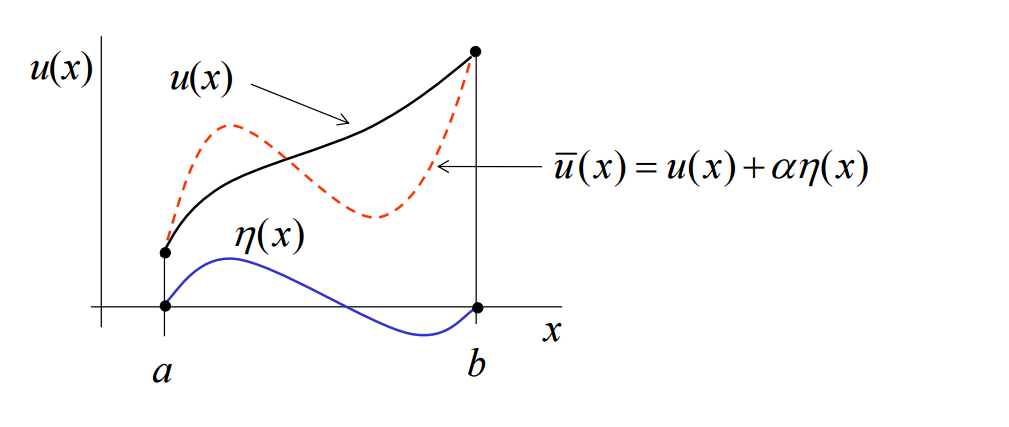
\includegraphics{../images/variation.PNG}
\end{frame}

\begin{frame}{euler lagrange}
\protect\hypertarget{euler-lagrange-3}{}
\begin{itemize}
\tightlist
\item
  We can take the derivative of \(\bar{y}\) to find
  \$\(\dot{\bar{y}} = \dot{y}(x) + \alpha \dot{\eta}(x)\)\$
\item
  This now gives
  \$\(I[\alpha] = \int_{x_0}^{x_1} F(x,\bar{y},\dot{\bar{y}})dx = \int_{x_0}^{x_1} F(x,y(x) + \alpha \eta(x),\dot{y}(x) + \alpha \dot{\eta}(x))dx\)\$
\item
  Once \emph{y}(\emph{x}) and \(\eta(x)\) are chosen, \emph{I} is a
  function of \$\alpha\$
\end{itemize}
\end{frame}

\begin{frame}{euler lagrange}
\protect\hypertarget{euler-lagrange-4}{}
\begin{itemize}
\tightlist
\item
  We find the stationary function by letting \$\frac{dI}{d \alpha} = 0\$
  \$\(\frac{dI}{d \alpha} = \int_{x_0}^{x_1} \frac{\partial F}{\partial \alpha} dx =  \int_{x_0}^{x_1} \left ( \frac{\partial F}{\partial \bar{y}}\frac{\partial \bar{y}}{\partial \alpha} +  \frac{\partial F}{\partial \dot{\bar{y}}}\frac{\partial \dot{\bar{y}}}{\partial \alpha}\right )dx\)\$
\item
  This simplifies to
  \$\(\int_{x_0}^{x_1} \left ( \frac{\partial F}{\partial \bar{y}}\eta +  \frac{\partial F}{\partial \dot{\bar{y}}}\dot{\eta}\right )dx\)\$
\end{itemize}
\end{frame}

\begin{frame}{euler lagrange}
\protect\hypertarget{euler-lagrange-5}{}
\begin{itemize}
\tightlist
\item
  Now we know that \emph{I} will be stationary when \(\alpha = 0\), in
  which case \(\bar{y}=y\), therefore we can write
  \$\(\int_{x_0}^{x_1} \left ( \frac{\partial F}{\partial y}\eta +  \frac{\partial F}{\partial \dot{y}}\dot{\eta}\right )dx = 0\)\$
\item
  And now we perform integration by parts on the second term
\end{itemize}
\end{frame}

\begin{frame}{integration by parts}
\protect\hypertarget{integration-by-parts}{}
\begin{itemize}
\item
  Recall that \$\(\int u dv = uv - \int v du\)\$
\item
  We choose
  \$\(\begin{aligned}  u &= \frac{\partial F}{\partial \dot{y}}\\  du &= \frac{d}{dx} \left( \frac{\partial F}{\partial y} \right)\\  v &= \eta(x)\\  dv &= \dot{\eta} dx \end{aligned}\)\$
\end{itemize}
\end{frame}

\begin{frame}{integration by parts}
\protect\hypertarget{integration-by-parts-1}{}
\begin{itemize}
\tightlist
\item
  This gives (for the second term)
  \$\(\int_{x_0}^{x_1} \frac{\partial F}{\partial \dot{y}}\dot{\eta} dx = \frac{\partial F}{\partial \dot{y}}\eta |_{x_0}^{x_1} - \int_{x_0}^{x_1} \frac{d}{dx} \left( \frac{\partial F}{\partial y} \right) \eta(x)\)\$
\item
  Combining with the original equation and simplifying gives
  \$\(\int_{x_0}^{x_1} \left [ \frac{\partial F}{\partial y} - \frac{d}{dx} \left( \frac{\partial F}{\partial y} \right) \right ]\eta dx + \frac{\partial F}{\partial \dot{y}}\eta |_{x_0}^{x_1} = 0\)\$
\end{itemize}
\end{frame}

\begin{frame}{euler lagrange}
\protect\hypertarget{euler-lagrange-6}{}
\begin{itemize}
\tightlist
\item
  We already know that \(\eta|_{x_0}^{x_1}=0\), so we only need concern
  ourselves with the terms inside the integral
\item
  Since this must be true for any arbitrary function, \(\eta\), we can
  say that
  \$\(\frac{\partial F}{\partial y} - \frac{d}{dx} \left( \frac{\partial F}{\partial y} \right) = 0\)\$
\item
  This is known as the Euler-Lagrange equation
\item
  A solution to the Euler-Lagrange equation is called an extremal, and
  an extremal which satisfies the boundary conditions is called a
  stationary function
\end{itemize}
\end{frame}

\begin{frame}{variations}
\protect\hypertarget{variations}{}
\begin{itemize}
\tightlist
\item
  In variational calculus, we define the first variation as
  \$\(\delta y = \bar{y} - y\)\$
\item
  Note: while the variation follows many of the same rules as
  differentiation, it does not correspond to any slope, since \(\eta\)
  is completely arbitrary
\end{itemize}
\end{frame}

\begin{frame}{variations}
\protect\hypertarget{variations-1}{}
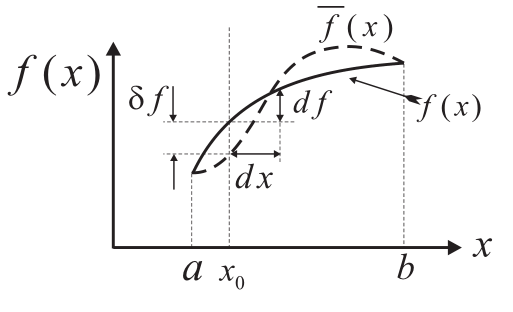
\includegraphics{../images/variations.PNG}
\end{frame}

\begin{frame}{variations}
\protect\hypertarget{variations-2}{}
\begin{itemize}
\tightlist
\item
  Variational laws are analogous to differentiation
\end{itemize}

\[\begin{aligned}
  \delta (F_1 F_2) &= F_1 \delta F_2 + \delta F_1 F_2\\
  \delta \left(\frac{F_1}{F_2} \right) &= \frac{F_2 \delta F_1 - F_1 \delta F_2}{F_2^2}
\end{aligned}\]

\begin{itemize}
\tightlist
\item
  The variation and derivative are commutative
\end{itemize}

\[\frac{d}{dx} (\delta u) = \delta \left(\frac{du}{dx}\right)\]

\begin{itemize}
\tightlist
\item
  Similarly, the variation is commutative with the integral
\end{itemize}

\[\delta \int F dx = \int \delta F dx\]
\end{frame}

\begin{frame}{variations}
\protect\hypertarget{variations-3}{}
\begin{itemize}
\tightlist
\item
  We can also take the variation of a functional
\end{itemize}

\[\Delta F = F(x,y + \alpha \eta, \dot{y} + \alpha \dot{\eta}) - F(x,y,\dot{y})\]

\begin{itemize}
\tightlist
\item
  Expanding this function via a Taylor series gives
\end{itemize}

\[\Delta F = \left [ F(x,y,\dot{y}) + \left( \delta y \frac{\partial F}{\partial y} + \delta \dot{y} \frac{\partial F}{\partial \dot{y}} + ... \right) \right]- F(x,y,\dot{y})\]

\begin{itemize}
\tightlist
\item
  And thus we call the variation of \emph{F}
\end{itemize}

\[\delta F = \frac{\partial F}{\partial y} \delta y + \frac{\partial F}{\partial \dot{y}} \delta \dot{y} + \epsilon_1\]

\begin{itemize}
\tightlist
\item
  Where \(\epsilon_1\) are terms of higher order than
  \(\sqrt{(\delta y)^2 + (\delta \dot{y})^2}\) and are neglected in the
  first variation
\end{itemize}
\end{frame}

\begin{frame}{variations}
\protect\hypertarget{variations-4}{}
\begin{itemize}
\tightlist
\item
  We can use variational notation to find the Euler-Lagrange equation
\end{itemize}

\[I[y] = \int_{x_0}^{x_1} F(x,y,\dot{y})dx\]

\begin{itemize}
\tightlist
\item
  and taking the variation
\end{itemize}

\[\delta I = \int_{x_0}^{x_1} \left[  \frac{\partial F}{\partial y} \delta y + \frac{\partial F}{\partial \dot{y}} \delta \dot{y}\right]dx = 0\]
\end{frame}

\begin{frame}{variations}
\protect\hypertarget{variations-5}{}
\begin{itemize}
\tightlist
\item
  Using integration by parts on the second term, as before, we find
\end{itemize}

\[\delta I = \int_{x_0}^{x_1} \left[  \frac{\partial F}{\partial y} - \frac{d}{dx}\left(\frac{\partial F}{\partial \dot{y}}\right) \right]\delta y dx = 0\]

\begin{itemize}
\tightlist
\item
  Since \(\delta y (x_0) = \delta y (x_1) = 0\)
\item
  Since this must be true for any arbitrary variation, we have
\end{itemize}

\[\frac{\partial F}{\partial y} - \frac{d}{dx}\left(\frac{\partial F}{\partial \dot{y}}\right)\]
\end{frame}

\begin{frame}{variations}
\protect\hypertarget{variations-6}{}
\begin{itemize}
\tightlist
\item
  If the functional, \emph{F}, does not depend on \emph{x} explicitly
  (i.e.~the only \emph{x} dependence comes from \emph{y}(\emph{x})) then
  we can say
\end{itemize}

\[\frac{d}{dx}\left( F - \dot{y} \frac{\partial F}{\partial \dot{y}}\right) = 0\]

\begin{itemize}
\tightlist
\item
  or, similarly
\end{itemize}

\[F - \dot{y} \frac{\partial F}{\partial \dot{y}} = C\]
\end{frame}

\begin{frame}{brachistochrone problem}
\protect\hypertarget{brachistochrone-problem}{}
\begin{itemize}
\tightlist
\item
  If we return now to Bernoulli's problem, we had found
\end{itemize}

\[t = \int_0^a \frac{\sqrt{1 + \dot{y}^2}}{\sqrt{2 g y}}dx\]

\begin{itemize}
\tightlist
\item
  Since this does not depend on \emph{x} explicitly, we can use the
  simpler form of the Euler-Lagrange equation.
\end{itemize}

\[F = \frac{\sqrt{1 + \dot{y}^2}}{\sqrt{2 g y}}\]

\begin{itemize}
\tightlist
\item
  with
\end{itemize}

\[F - \dot{y} \frac{\partial F}{\partial \dot{y}} = C\]
\end{frame}

\begin{frame}{brachistochrone problem}
\protect\hypertarget{brachistochrone-problem-1}{}
\begin{itemize}
\tightlist
\item
  Computing the partial derivative we find
\end{itemize}

\[\frac{\partial F}{\partial \dot{y}} = \frac{\dot{y}}{\sqrt{2 g y}\sqrt{1 + \dot{y}^2}}\]

\begin{itemize}
\tightlist
\item
  Which gives in the Euler-Lagrange equation
\end{itemize}

\[\frac{\sqrt{1 + \dot{y}^2}}{\sqrt{2 g y}} - \frac{\dot{y}^2}{\sqrt{2 g y}\sqrt{1 + \dot{y}^2}} = C\]
\end{frame}

\begin{frame}{brachistrochrone problem}
\protect\hypertarget{brachistrochrone-problem}{}
\begin{itemize}
\tightlist
\item
  Simplifying gives
\end{itemize}

\[\frac{1}{\sqrt{2 g y}\sqrt{1 + \dot{y}^2}} = C\]

\begin{itemize}
\tightlist
\item
  We can square both sides and lump constants together
\end{itemize}

\[y(1+\dot{y}^2) = \frac{1}{2gc^2} = c_1\]

\begin{itemize}
\tightlist
\item
  And solving for \(\dot{y}\), taking only the positive solution
\end{itemize}

\[\dot{y} = \frac{\sqrt{c_1-y}}{\sqrt{y}}\]
\end{frame}

\begin{frame}{brachistochrone problem}
\protect\hypertarget{brachistochrone-problem-2}{}
\begin{itemize}
\tightlist
\item
  The Brachistochrone problem can be solved using parametric equations
\end{itemize}

\[\begin{aligned}
  x &= k^2 (\theta - \sin\theta)\\
  y &= k^2 (1-\cos\theta)
\end{aligned}\]
\end{frame}

\begin{frame}{example}
\protect\hypertarget{example-1}{}
\begin{itemize}
\tightlist
\item
  We can also use variational calculus to prove that the shortest
  distance between to points is a straight line
\item
  The distance along a curve is given by
\end{itemize}

\[L = \int_a^b ds\]

\begin{itemize}
\tightlist
\item
  Where \(ds = \sqrt{dx^2 + dy^2} = \sqrt{1+ \dot{y}^2}dx\)
\item
  So we can find the minimum of the functional
\end{itemize}

\[I[y] = \int_a^b \sqrt{1+ \dot{y}^2}dx\]
\end{frame}

\begin{frame}{group problems}
\protect\hypertarget{group-problems}{}
\begin{itemize}
\tightlist
\item
  Find the Euler-Lagrange equation for
\end{itemize}

\[I[y] = \int y\sqrt{1+\dot{y}^2} dx\]

\begin{itemize}
\tightlist
\item
  Find the Euler-Lagrange equation for
\end{itemize}

\[I[y] = \int [\dot{y}^2 + y^2 + 2xy] dx\]
\end{frame}

\begin{frame}{next class}
\protect\hypertarget{next-class}{}
\begin{itemize}
\tightlist
\item
  Boundary conditions
\item
  Multi-variate variational calculus
\item
  Approximate solutions
\item
  Variational Asymptotic Method
\end{itemize}
\end{frame}

\end{document}
